% Options for packages loaded elsewhere
\PassOptionsToPackage{unicode}{hyperref}
\PassOptionsToPackage{hyphens}{url}
%
\documentclass[
]{article}
\usepackage{amsmath,amssymb}
\usepackage{lmodern}
\usepackage{iftex}
\ifPDFTeX
  \usepackage[T1]{fontenc}
  \usepackage[utf8]{inputenc}
  \usepackage{textcomp} % provide euro and other symbols
\else % if luatex or xetex
  \usepackage{unicode-math}
  \defaultfontfeatures{Scale=MatchLowercase}
  \defaultfontfeatures[\rmfamily]{Ligatures=TeX,Scale=1}
\fi
% Use upquote if available, for straight quotes in verbatim environments
\IfFileExists{upquote.sty}{\usepackage{upquote}}{}
\IfFileExists{microtype.sty}{% use microtype if available
  \usepackage[]{microtype}
  \UseMicrotypeSet[protrusion]{basicmath} % disable protrusion for tt fonts
}{}
\makeatletter
\@ifundefined{KOMAClassName}{% if non-KOMA class
  \IfFileExists{parskip.sty}{%
    \usepackage{parskip}
  }{% else
    \setlength{\parindent}{0pt}
    \setlength{\parskip}{6pt plus 2pt minus 1pt}}
}{% if KOMA class
  \KOMAoptions{parskip=half}}
\makeatother
\usepackage{xcolor}
\usepackage[margin=1in]{geometry}
\usepackage{color}
\usepackage{fancyvrb}
\newcommand{\VerbBar}{|}
\newcommand{\VERB}{\Verb[commandchars=\\\{\}]}
\DefineVerbatimEnvironment{Highlighting}{Verbatim}{commandchars=\\\{\}}
% Add ',fontsize=\small' for more characters per line
\usepackage{framed}
\definecolor{shadecolor}{RGB}{248,248,248}
\newenvironment{Shaded}{\begin{snugshade}}{\end{snugshade}}
\newcommand{\AlertTok}[1]{\textcolor[rgb]{0.94,0.16,0.16}{#1}}
\newcommand{\AnnotationTok}[1]{\textcolor[rgb]{0.56,0.35,0.01}{\textbf{\textit{#1}}}}
\newcommand{\AttributeTok}[1]{\textcolor[rgb]{0.77,0.63,0.00}{#1}}
\newcommand{\BaseNTok}[1]{\textcolor[rgb]{0.00,0.00,0.81}{#1}}
\newcommand{\BuiltInTok}[1]{#1}
\newcommand{\CharTok}[1]{\textcolor[rgb]{0.31,0.60,0.02}{#1}}
\newcommand{\CommentTok}[1]{\textcolor[rgb]{0.56,0.35,0.01}{\textit{#1}}}
\newcommand{\CommentVarTok}[1]{\textcolor[rgb]{0.56,0.35,0.01}{\textbf{\textit{#1}}}}
\newcommand{\ConstantTok}[1]{\textcolor[rgb]{0.00,0.00,0.00}{#1}}
\newcommand{\ControlFlowTok}[1]{\textcolor[rgb]{0.13,0.29,0.53}{\textbf{#1}}}
\newcommand{\DataTypeTok}[1]{\textcolor[rgb]{0.13,0.29,0.53}{#1}}
\newcommand{\DecValTok}[1]{\textcolor[rgb]{0.00,0.00,0.81}{#1}}
\newcommand{\DocumentationTok}[1]{\textcolor[rgb]{0.56,0.35,0.01}{\textbf{\textit{#1}}}}
\newcommand{\ErrorTok}[1]{\textcolor[rgb]{0.64,0.00,0.00}{\textbf{#1}}}
\newcommand{\ExtensionTok}[1]{#1}
\newcommand{\FloatTok}[1]{\textcolor[rgb]{0.00,0.00,0.81}{#1}}
\newcommand{\FunctionTok}[1]{\textcolor[rgb]{0.00,0.00,0.00}{#1}}
\newcommand{\ImportTok}[1]{#1}
\newcommand{\InformationTok}[1]{\textcolor[rgb]{0.56,0.35,0.01}{\textbf{\textit{#1}}}}
\newcommand{\KeywordTok}[1]{\textcolor[rgb]{0.13,0.29,0.53}{\textbf{#1}}}
\newcommand{\NormalTok}[1]{#1}
\newcommand{\OperatorTok}[1]{\textcolor[rgb]{0.81,0.36,0.00}{\textbf{#1}}}
\newcommand{\OtherTok}[1]{\textcolor[rgb]{0.56,0.35,0.01}{#1}}
\newcommand{\PreprocessorTok}[1]{\textcolor[rgb]{0.56,0.35,0.01}{\textit{#1}}}
\newcommand{\RegionMarkerTok}[1]{#1}
\newcommand{\SpecialCharTok}[1]{\textcolor[rgb]{0.00,0.00,0.00}{#1}}
\newcommand{\SpecialStringTok}[1]{\textcolor[rgb]{0.31,0.60,0.02}{#1}}
\newcommand{\StringTok}[1]{\textcolor[rgb]{0.31,0.60,0.02}{#1}}
\newcommand{\VariableTok}[1]{\textcolor[rgb]{0.00,0.00,0.00}{#1}}
\newcommand{\VerbatimStringTok}[1]{\textcolor[rgb]{0.31,0.60,0.02}{#1}}
\newcommand{\WarningTok}[1]{\textcolor[rgb]{0.56,0.35,0.01}{\textbf{\textit{#1}}}}
\usepackage{graphicx}
\makeatletter
\def\maxwidth{\ifdim\Gin@nat@width>\linewidth\linewidth\else\Gin@nat@width\fi}
\def\maxheight{\ifdim\Gin@nat@height>\textheight\textheight\else\Gin@nat@height\fi}
\makeatother
% Scale images if necessary, so that they will not overflow the page
% margins by default, and it is still possible to overwrite the defaults
% using explicit options in \includegraphics[width, height, ...]{}
\setkeys{Gin}{width=\maxwidth,height=\maxheight,keepaspectratio}
% Set default figure placement to htbp
\makeatletter
\def\fps@figure{htbp}
\makeatother
\setlength{\emergencystretch}{3em} % prevent overfull lines
\providecommand{\tightlist}{%
  \setlength{\itemsep}{0pt}\setlength{\parskip}{0pt}}
\setcounter{secnumdepth}{-\maxdimen} % remove section numbering
\ifLuaTeX
  \usepackage{selnolig}  % disable illegal ligatures
\fi
\IfFileExists{bookmark.sty}{\usepackage{bookmark}}{\usepackage{hyperref}}
\IfFileExists{xurl.sty}{\usepackage{xurl}}{} % add URL line breaks if available
\urlstyle{same} % disable monospaced font for URLs
\hypersetup{
  pdftitle={Report},
  hidelinks,
  pdfcreator={LaTeX via pandoc}}

\title{Report}
\author{}
\date{\vspace{-2.5em}2022-09-19}

\begin{document}
\maketitle

\hypertarget{mixed-effect-models}{%
\subsection{Mixed-effect models}\label{mixed-effect-models}}

\hypertarget{here-are-some-mixed-effect-of-the-data-collected-from-the-vr-experiments}{%
\subsubsection{Here are some mixed effect of the data collected from the
VR
experiments}\label{here-are-some-mixed-effect-of-the-data-collected-from-the-vr-experiments}}

Effects:

--\textgreater{} IsIntroducer: If this is the first time the director is
seeing the target

--\textgreater{} TIME: The duration of the game

--\textgreater{} PAIR: Pair number

--\textgreater{} TARGET: Target word that needs to be guessed

--\textgreater{} GAME: Game number

--\textgreater{} condition: modified or normal

--\textgreater{} PARTICIPANT: each individual

\begin{verbatim}
## Loading required package: Matrix
\end{verbatim}

\hypertarget{standard-deviation}{%
\subsection{Standard deviation}\label{standard-deviation}}

\hypertarget{these-linear-mixed-effect-models-investigates-the-effect-of-condition-on-the-standard-deviation-of-the-z-axis-and-the-x-axis.}{%
\subsubsection{These linear mixed-effect models investigates the effect
of condition on the standard deviation of the z-axis and the
x-axis.}\label{these-linear-mixed-effect-models-investigates-the-effect-of-condition-on-the-standard-deviation-of-the-z-axis-and-the-x-axis.}}

\begin{Shaded}
\begin{Highlighting}[]
\NormalTok{lmodel2B }\OtherTok{=}  \FunctionTok{lmer}\NormalTok{ (sdz }\SpecialCharTok{\textasciitilde{}}\NormalTok{   condition }\SpecialCharTok{+}\NormalTok{ (condition}\SpecialCharTok{|}\NormalTok{PAIR) }\SpecialCharTok{+}\NormalTok{ (}\DecValTok{1} \SpecialCharTok{|}\NormalTok{ PARTICIPANT) }\SpecialCharTok{+}\NormalTok{ (condition}\SpecialCharTok{|}\NormalTok{TARGET))}
\end{Highlighting}
\end{Shaded}

\begin{verbatim}
## boundary (singular) fit: see help('isSingular')
\end{verbatim}

\begin{Shaded}
\begin{Highlighting}[]
\FunctionTok{AIC}\NormalTok{(lmodel2B)}
\end{Highlighting}
\end{Shaded}

\begin{verbatim}
## [1] -2396.833
\end{verbatim}

\begin{Shaded}
\begin{Highlighting}[]
\NormalTok{model2Bgraph }\OtherTok{=} \FunctionTok{ggpredict}\NormalTok{(lmodel2B,}\FunctionTok{c}\NormalTok{(}\StringTok{"condition"}\NormalTok{))}
\FunctionTok{plot}\NormalTok{(model2Bgraph)}
\end{Highlighting}
\end{Shaded}

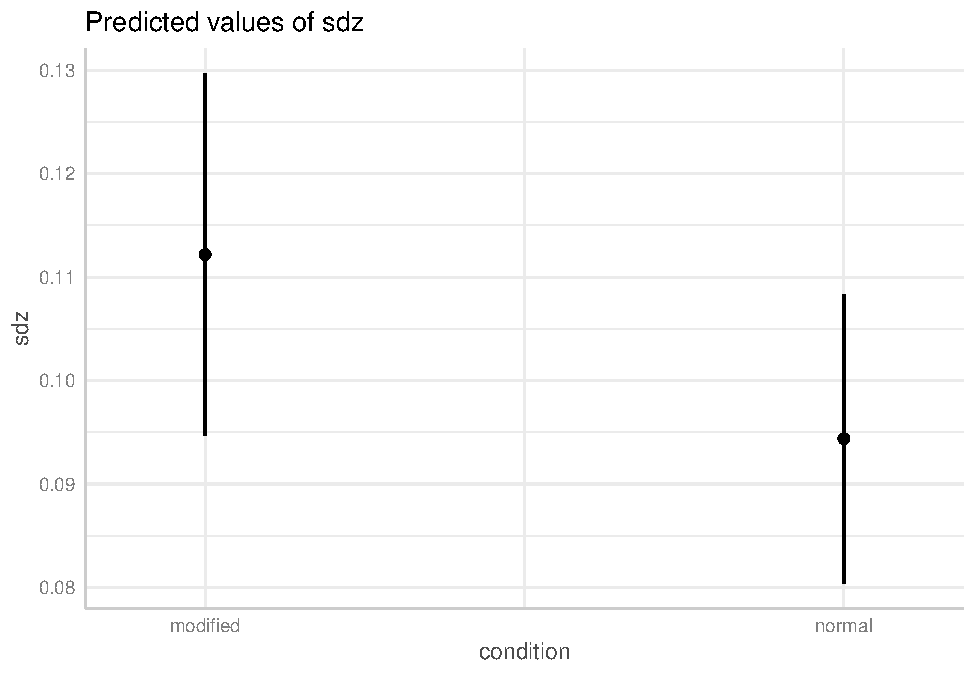
\includegraphics{Report_files/figure-latex/pressure-1.pdf}

\begin{Shaded}
\begin{Highlighting}[]
\NormalTok{lmodel2C }\OtherTok{=}  \FunctionTok{lmer}\NormalTok{ (sdx }\SpecialCharTok{\textasciitilde{}}\NormalTok{   condition }\SpecialCharTok{+}\NormalTok{ (condition}\SpecialCharTok{|}\NormalTok{PAIR) }\SpecialCharTok{+}\NormalTok{ (}\DecValTok{1} \SpecialCharTok{|}\NormalTok{ PARTICIPANT) }\SpecialCharTok{+}\NormalTok{(condition}\SpecialCharTok{|}\NormalTok{TARGET))}
\FunctionTok{AIC}\NormalTok{(lmodel2C)}
\end{Highlighting}
\end{Shaded}

\begin{verbatim}
## [1] -1938.964
\end{verbatim}

\begin{Shaded}
\begin{Highlighting}[]
\NormalTok{model2Cgraph }\OtherTok{=} \FunctionTok{ggpredict}\NormalTok{(lmodel2C,}\FunctionTok{c}\NormalTok{(}\StringTok{"condition"}\NormalTok{))}
\FunctionTok{plot}\NormalTok{(model2Cgraph)}
\end{Highlighting}
\end{Shaded}

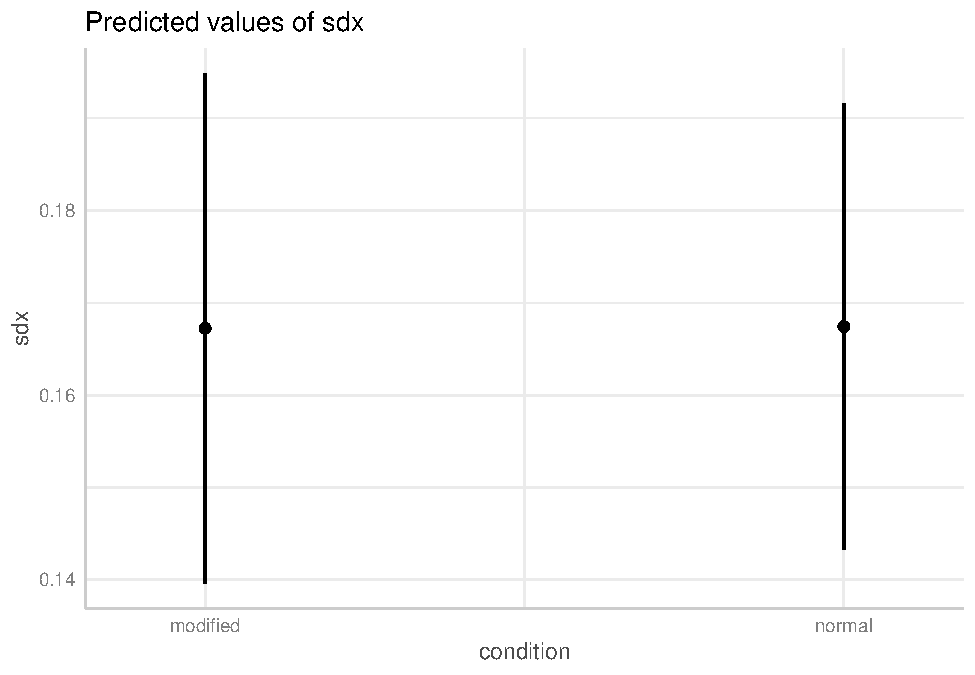
\includegraphics{Report_files/figure-latex/pressure-2.pdf}

\hypertarget{because-i-switched-the-x-axis-with-the-z-axis-in-the-modified-group-i-also-want-to-see-if-more-movement-on-the-z-axis-is-caused-by-less-movement-on-the-x-axis-for-the-modified-group}{%
\subsubsection{Because I switched the x-axis with the z-axis in the
modified group, I also want to see if more movement on the z-axis is
caused by less movement on the x-axis ( for the modified
group):}\label{because-i-switched-the-x-axis-with-the-z-axis-in-the-modified-group-i-also-want-to-see-if-more-movement-on-the-z-axis-is-caused-by-less-movement-on-the-x-axis-for-the-modified-group}}

\begin{Shaded}
\begin{Highlighting}[]
\NormalTok{lmodel12 }\OtherTok{=}  \FunctionTok{lmer}\NormalTok{ (sdz }\SpecialCharTok{\textasciitilde{}}\NormalTok{   sdx}\SpecialCharTok{*}\NormalTok{condition }\SpecialCharTok{+}\NormalTok{ (sdx}\SpecialCharTok{*}\NormalTok{condition}\SpecialCharTok{|}\NormalTok{PAIR) }\SpecialCharTok{+}\NormalTok{ (}\DecValTok{1} \SpecialCharTok{|}\NormalTok{ PARTICIPANT) }\SpecialCharTok{+}\NormalTok{ (sdx}\SpecialCharTok{*}\NormalTok{condition}\SpecialCharTok{|}\NormalTok{TARGET))}
\end{Highlighting}
\end{Shaded}

\begin{verbatim}
## boundary (singular) fit: see help('isSingular')
\end{verbatim}

\begin{Shaded}
\begin{Highlighting}[]
\FunctionTok{AIC}\NormalTok{(lmodel12)}
\end{Highlighting}
\end{Shaded}

\begin{verbatim}
## [1] -2498.117
\end{verbatim}

\begin{Shaded}
\begin{Highlighting}[]
\NormalTok{model12graph }\OtherTok{=} \FunctionTok{ggpredict}\NormalTok{(lmodel12,}\FunctionTok{c}\NormalTok{(}\StringTok{"sdx"}\NormalTok{,}\StringTok{"condition"}\NormalTok{))}
\FunctionTok{plot}\NormalTok{(model12graph)}
\end{Highlighting}
\end{Shaded}

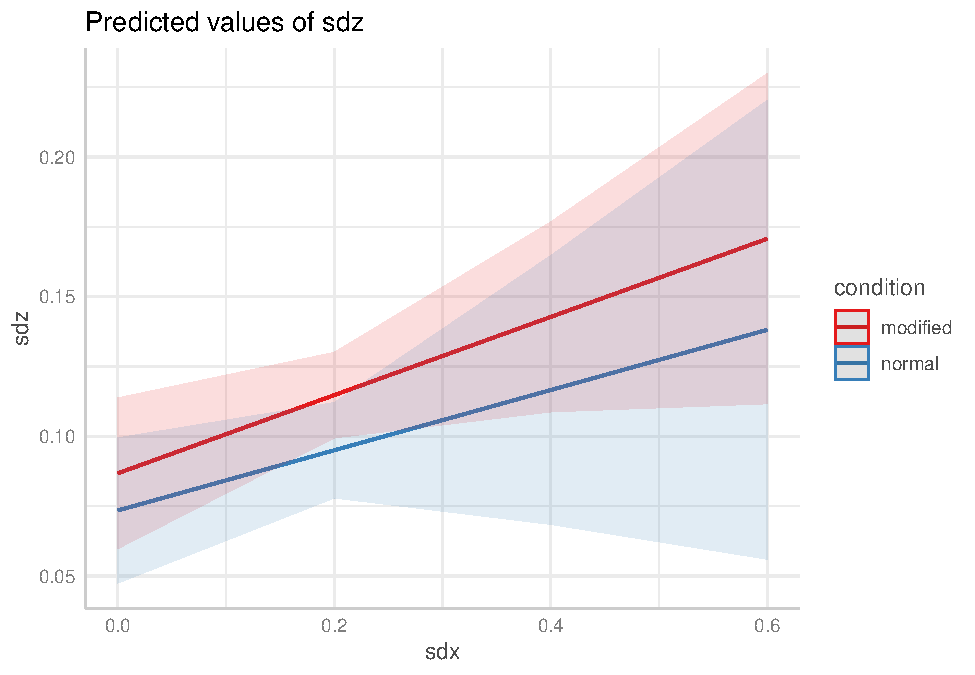
\includegraphics{Report_files/figure-latex/pressure2-1.pdf}

\hypertarget{i-also-checked-the-effect-that-introducer-have-on-the-the-z-axis-in-combination-with-other-fixed-effect-like-win-and-condition}{%
\subsubsection{I also checked the effect that introducer have on the the
z-axis (in combination with other fixed effect like Win and condition)
:}\label{i-also-checked-the-effect-that-introducer-have-on-the-the-z-axis-in-combination-with-other-fixed-effect-like-win-and-condition}}

\begin{Shaded}
\begin{Highlighting}[]
\NormalTok{lmodel }\OtherTok{=}  \FunctionTok{lmer}\NormalTok{ (sdz }\SpecialCharTok{\textasciitilde{}}\NormalTok{   IsIntroducer }\SpecialCharTok{+}\NormalTok{ (IsIntroducer}\SpecialCharTok{|}\NormalTok{PAIR) }\SpecialCharTok{+}\NormalTok{ (}\DecValTok{1} \SpecialCharTok{|}\NormalTok{ PARTICIPANT) }\SpecialCharTok{+}\NormalTok{ (IsIntroducer}\SpecialCharTok{|}\NormalTok{TARGET))}
\end{Highlighting}
\end{Shaded}

\begin{verbatim}
## boundary (singular) fit: see help('isSingular')
\end{verbatim}

\begin{Shaded}
\begin{Highlighting}[]
\NormalTok{lmodel3 }\OtherTok{=}  \FunctionTok{lmer}\NormalTok{ (sdz }\SpecialCharTok{\textasciitilde{}}\NormalTok{   condition}\SpecialCharTok{+}\NormalTok{IsIntroducer }\SpecialCharTok{+}\NormalTok{ (condition}\SpecialCharTok{+}\NormalTok{IsIntroducer}\SpecialCharTok{|}\NormalTok{PAIR) }\SpecialCharTok{+}\NormalTok{ (}\DecValTok{1} \SpecialCharTok{|}\NormalTok{ PARTICIPANT) }\SpecialCharTok{+}\NormalTok{ (condition}\SpecialCharTok{+}\NormalTok{IsIntroducer}\SpecialCharTok{|}\NormalTok{TARGET))}
\end{Highlighting}
\end{Shaded}

\begin{verbatim}
## boundary (singular) fit: see help('isSingular')
\end{verbatim}

\begin{Shaded}
\begin{Highlighting}[]
\NormalTok{lmodel4 }\OtherTok{=}  \FunctionTok{lmer}\NormalTok{ (sdz }\SpecialCharTok{\textasciitilde{}}\NormalTok{   condition}\SpecialCharTok{*}\NormalTok{IsIntroducer }\SpecialCharTok{+}\NormalTok{ (condition}\SpecialCharTok{*}\NormalTok{IsIntroducer}\SpecialCharTok{|}\NormalTok{PAIR) }\SpecialCharTok{+}\NormalTok{ (}\DecValTok{1} \SpecialCharTok{|}\NormalTok{ PARTICIPANT) }\SpecialCharTok{+}\NormalTok{ (condition}\SpecialCharTok{*}\NormalTok{IsIntroducer}\SpecialCharTok{|}\NormalTok{TARGET))}
\end{Highlighting}
\end{Shaded}

\begin{verbatim}
## boundary (singular) fit: see help('isSingular')
\end{verbatim}

\begin{Shaded}
\begin{Highlighting}[]
\NormalTok{lmodel5 }\OtherTok{=}  \FunctionTok{lmer}\NormalTok{ (sdz }\SpecialCharTok{\textasciitilde{}}\NormalTok{   Win }\SpecialCharTok{+}\NormalTok{ (Win}\SpecialCharTok{|}\NormalTok{PAIR) }\SpecialCharTok{+}\NormalTok{ (}\DecValTok{1} \SpecialCharTok{|}\NormalTok{ PARTICIPANT) }\SpecialCharTok{+}\NormalTok{ (Win}\SpecialCharTok{|}\NormalTok{TARGET))}
\NormalTok{lmodel6 }\OtherTok{=}  \FunctionTok{lmer}\NormalTok{ (sdz }\SpecialCharTok{\textasciitilde{}}\NormalTok{   Win}\SpecialCharTok{+}\NormalTok{IsIntroducer }\SpecialCharTok{+}\NormalTok{ (Win}\SpecialCharTok{+}\NormalTok{IsIntroducer}\SpecialCharTok{|}\NormalTok{PAIR) }\SpecialCharTok{+}\NormalTok{ (}\DecValTok{1} \SpecialCharTok{|}\NormalTok{ PARTICIPANT) }\SpecialCharTok{+}\NormalTok{ (Win}\SpecialCharTok{+}\NormalTok{IsIntroducer}\SpecialCharTok{|}\NormalTok{TARGET))}
\end{Highlighting}
\end{Shaded}

\begin{verbatim}
## boundary (singular) fit: see help('isSingular')
\end{verbatim}

\begin{Shaded}
\begin{Highlighting}[]
\NormalTok{lmodel7 }\OtherTok{=}  \FunctionTok{lmer}\NormalTok{ (sdz }\SpecialCharTok{\textasciitilde{}}\NormalTok{   Win}\SpecialCharTok{*}\NormalTok{IsIntroducer }\SpecialCharTok{+}\NormalTok{ (Win}\SpecialCharTok{*}\NormalTok{IsIntroducer}\SpecialCharTok{|}\NormalTok{PAIR) }\SpecialCharTok{+}\NormalTok{ (}\DecValTok{1} \SpecialCharTok{|}\NormalTok{ PARTICIPANT) }\SpecialCharTok{+}\NormalTok{ (Win}\SpecialCharTok{*}\NormalTok{IsIntroducer}\SpecialCharTok{|}\NormalTok{TARGET))}
\end{Highlighting}
\end{Shaded}

\begin{verbatim}
## boundary (singular) fit: see help('isSingular')
\end{verbatim}

\begin{Shaded}
\begin{Highlighting}[]
\FunctionTok{AIC}\NormalTok{(lmodel,lmodel3,lmodel4,lmodel5,lmodel6,lmodel7)}
\end{Highlighting}
\end{Shaded}

\begin{verbatim}
##         df       AIC
## lmodel  10 -2397.441
## lmodel3 17 -2388.702
## lmodel4 26 -2365.219
## lmodel5 10 -2398.221
## lmodel6 17 -2393.710
## lmodel7 26 -2404.400
\end{verbatim}

\begin{Shaded}
\begin{Highlighting}[]
\CommentTok{\#Model lmodel7 seems to be the best performing model, based on the AIC score.}
\NormalTok{modelgraph }\OtherTok{=} \FunctionTok{ggpredict}\NormalTok{(lmodel7,}\FunctionTok{c}\NormalTok{(}\StringTok{"IsIntroducer"}\NormalTok{,}\StringTok{"Win"}\NormalTok{))}
\FunctionTok{plot}\NormalTok{(modelgraph)}
\end{Highlighting}
\end{Shaded}

\includegraphics{Report_files/figure-latex/pressure22-1.pdf}

\begin{Shaded}
\begin{Highlighting}[]
\NormalTok{P1}\OtherTok{\textless{}{-}}\FunctionTok{read.csv}\NormalTok{(}\StringTok{"data\_P1\_TpR.csv"}\NormalTok{)}
\NormalTok{P2}\OtherTok{\textless{}{-}}\FunctionTok{read.csv}\NormalTok{(}\StringTok{"data\_P2\_TpR.csv"}\NormalTok{)}

\NormalTok{P1\_sd}\OtherTok{\textless{}{-}}\FunctionTok{read.csv}\NormalTok{(}\StringTok{"data\_P1\_SD.csv"}\NormalTok{)}

\NormalTok{P2\_sd}\OtherTok{\textless{}{-}}\FunctionTok{read.csv}\NormalTok{(}\StringTok{"data\_P2\_SD.csv"}\NormalTok{)}
\NormalTok{P2\_sd}\SpecialCharTok{$}\NormalTok{Time }\OtherTok{\textless{}{-}}\NormalTok{ P2}\SpecialCharTok{$}\NormalTok{Time}

\NormalTok{success }\OtherTok{\textless{}{-}} \FunctionTok{as.numeric}\NormalTok{(P2\_sd}\SpecialCharTok{$}\NormalTok{Success)}
\NormalTok{condition}\OtherTok{\textless{}{-}}\FunctionTok{as.factor}\NormalTok{(P2\_sd}\SpecialCharTok{$}\NormalTok{Condtion)}
\NormalTok{TIME }\OtherTok{\textless{}{-}}\FunctionTok{round}\NormalTok{(P2\_sd}\SpecialCharTok{$}\NormalTok{Time}\SpecialCharTok{/}\DecValTok{1000}\NormalTok{)}
\NormalTok{PAIR }\OtherTok{\textless{}{-}} \FunctionTok{as.factor}\NormalTok{(P2\_sd}\SpecialCharTok{$}\NormalTok{Pair)}
\NormalTok{TARGET}\OtherTok{\textless{}{-}} \FunctionTok{as.factor}\NormalTok{(P2\_sd}\SpecialCharTok{$}\NormalTok{Target)}
\NormalTok{IsIntroducer }\OtherTok{\textless{}{-}}\FunctionTok{as.factor}\NormalTok{(P2\_sd}\SpecialCharTok{$}\NormalTok{Introducer)}
\NormalTok{GAME}\OtherTok{\textless{}{-}}\NormalTok{ P2\_sd}\SpecialCharTok{$}\NormalTok{Game}
\NormalTok{sdz}\OtherTok{\textless{}{-}}\NormalTok{P2\_sd}\SpecialCharTok{$}\NormalTok{Z}
\NormalTok{sdx}\OtherTok{\textless{}{-}}\NormalTok{P2\_sd}\SpecialCharTok{$}\NormalTok{X}
\NormalTok{sdy}\OtherTok{\textless{}{-}}\NormalTok{P2\_sd}\SpecialCharTok{$}\NormalTok{Y}
\end{Highlighting}
\end{Shaded}

\hypertarget{success}{%
\subsection{Success}\label{success}}

\hypertarget{here-are-some-models-attempting-to-predict-the-success-rate-using-various-fixed-effects}{%
\subsubsection{Here are some models attempting to predict the success
rate using various fixed
effects}\label{here-are-some-models-attempting-to-predict-the-success-rate-using-various-fixed-effects}}

\begin{Shaded}
\begin{Highlighting}[]
\NormalTok{model9 }\OtherTok{=} \FunctionTok{glmer}\NormalTok{( success }\SpecialCharTok{\textasciitilde{}}\NormalTok{ IsIntroducer}\SpecialCharTok{+}\NormalTok{TIME }\SpecialCharTok{+}\NormalTok{ (IsIntroducer}\SpecialCharTok{+}\NormalTok{TIME}\SpecialCharTok{|}\NormalTok{PAIR) }\SpecialCharTok{+}\NormalTok{ (IsIntroducer}\SpecialCharTok{+}\NormalTok{TIME}\SpecialCharTok{|}\NormalTok{TARGET),}\AttributeTok{family =} \FunctionTok{binomial}\NormalTok{(}\AttributeTok{link =} \StringTok{"logit"}\NormalTok{),}\AttributeTok{control =} \FunctionTok{glmerControl}\NormalTok{(}\AttributeTok{optimizer =}\StringTok{\textquotesingle{}optimx\textquotesingle{}}\NormalTok{, }\AttributeTok{optCtrl=}\FunctionTok{list}\NormalTok{(}\AttributeTok{method=}\StringTok{\textquotesingle{}nlminb\textquotesingle{}}\NormalTok{)))}
\NormalTok{model8 }\OtherTok{=} \FunctionTok{glmer}\NormalTok{( success }\SpecialCharTok{\textasciitilde{}}\NormalTok{ IsIntroducer }\SpecialCharTok{+}\NormalTok{ (IsIntroducer}\SpecialCharTok{|}\NormalTok{PAIR) }\SpecialCharTok{+}\NormalTok{ (IsIntroducer}\SpecialCharTok{|}\NormalTok{TARGET),}\AttributeTok{family =} \FunctionTok{binomial}\NormalTok{(}\AttributeTok{link =} \StringTok{"logit"}\NormalTok{),}\AttributeTok{control =} \FunctionTok{glmerControl}\NormalTok{(}\AttributeTok{optimizer =}\StringTok{\textquotesingle{}optimx\textquotesingle{}}\NormalTok{, }\AttributeTok{optCtrl=}\FunctionTok{list}\NormalTok{(}\AttributeTok{method=}\StringTok{\textquotesingle{}nlminb\textquotesingle{}}\NormalTok{)))}
\NormalTok{model7 }\OtherTok{=} \FunctionTok{glmer}\NormalTok{( success }\SpecialCharTok{\textasciitilde{}}\NormalTok{ GAME}\SpecialCharTok{*}\NormalTok{TIME }\SpecialCharTok{+}\NormalTok{ (GAME}\SpecialCharTok{*}\NormalTok{TIME}\SpecialCharTok{|}\NormalTok{PAIR) }\SpecialCharTok{+}\NormalTok{ (GAME}\SpecialCharTok{*}\NormalTok{TIME}\SpecialCharTok{|}\NormalTok{TARGET),}\AttributeTok{family =} \FunctionTok{binomial}\NormalTok{(}\AttributeTok{link =} \StringTok{"logit"}\NormalTok{),}\AttributeTok{control =} \FunctionTok{glmerControl}\NormalTok{(}\AttributeTok{optimizer =}\StringTok{\textquotesingle{}optimx\textquotesingle{}}\NormalTok{, }\AttributeTok{optCtrl=}\FunctionTok{list}\NormalTok{(}\AttributeTok{method=}\StringTok{\textquotesingle{}nlminb\textquotesingle{}}\NormalTok{)))}
\NormalTok{model6 }\OtherTok{=} \FunctionTok{glmer}\NormalTok{( success }\SpecialCharTok{\textasciitilde{}}\NormalTok{ GAME}\SpecialCharTok{+}\NormalTok{TIME }\SpecialCharTok{+}\NormalTok{ (GAME}\SpecialCharTok{+}\NormalTok{TIME}\SpecialCharTok{|}\NormalTok{PAIR) }\SpecialCharTok{+}\NormalTok{ (GAME}\SpecialCharTok{+}\NormalTok{TIME}\SpecialCharTok{|}\NormalTok{TARGET),}\AttributeTok{family =} \FunctionTok{binomial}\NormalTok{(}\AttributeTok{link =} \StringTok{"logit"}\NormalTok{))}
\NormalTok{model5 }\OtherTok{=} \FunctionTok{glmer}\NormalTok{( success }\SpecialCharTok{\textasciitilde{}}\NormalTok{ GAME }\SpecialCharTok{+}\NormalTok{ (GAME}\SpecialCharTok{|}\NormalTok{PAIR) }\SpecialCharTok{+}\NormalTok{ (GAME}\SpecialCharTok{|}\NormalTok{TARGET),}\AttributeTok{family =} \FunctionTok{binomial}\NormalTok{(}\AttributeTok{link =} \StringTok{"logit"}\NormalTok{))}
\NormalTok{model4 }\OtherTok{=} \FunctionTok{glmer}\NormalTok{( success }\SpecialCharTok{\textasciitilde{}}\NormalTok{ condition }\SpecialCharTok{*}\NormalTok{ TIME }\SpecialCharTok{+}\NormalTok{ (condition}\SpecialCharTok{*}\NormalTok{TIME}\SpecialCharTok{|}\NormalTok{PAIR) }\SpecialCharTok{+}\NormalTok{ (condition }\SpecialCharTok{*}\NormalTok{TIME}\SpecialCharTok{|}\NormalTok{ TARGET), }\AttributeTok{control =} \FunctionTok{glmerControl}\NormalTok{(}\AttributeTok{optimizer =}\StringTok{\textquotesingle{}optimx\textquotesingle{}}\NormalTok{, }\AttributeTok{optCtrl=}\FunctionTok{list}\NormalTok{(}\AttributeTok{method=}\StringTok{\textquotesingle{}nlminb\textquotesingle{}}\NormalTok{)), }\AttributeTok{family =} \FunctionTok{binomial}\NormalTok{(}\AttributeTok{link =} \StringTok{"logit"}\NormalTok{))}
\NormalTok{model3 }\OtherTok{=} \FunctionTok{glmer}\NormalTok{( success }\SpecialCharTok{\textasciitilde{}}\NormalTok{ condition }\SpecialCharTok{+}\NormalTok{ TIME }\SpecialCharTok{+}\NormalTok{ (condition}\SpecialCharTok{+}\NormalTok{TIME}\SpecialCharTok{|}\NormalTok{PAIR) }\SpecialCharTok{+}\NormalTok{ (condition }\SpecialCharTok{+}\NormalTok{TIME}\SpecialCharTok{|}\NormalTok{ TARGET), }\AttributeTok{control =} \FunctionTok{glmerControl}\NormalTok{(}\AttributeTok{optimizer =}\StringTok{\textquotesingle{}optimx\textquotesingle{}}\NormalTok{, }\AttributeTok{optCtrl=}\FunctionTok{list}\NormalTok{(}\AttributeTok{method=}\StringTok{\textquotesingle{}nlminb\textquotesingle{}}\NormalTok{)),  }\AttributeTok{family =} \FunctionTok{binomial}\NormalTok{(}\AttributeTok{link =} \StringTok{"logit"}\NormalTok{))}
\NormalTok{model2B }\OtherTok{=} \FunctionTok{glmer}\NormalTok{( success }\SpecialCharTok{\textasciitilde{}}\NormalTok{ condition }\SpecialCharTok{+}\NormalTok{ (condition}\SpecialCharTok{|}\NormalTok{PAIR) }\SpecialCharTok{+}\NormalTok{ (condition}\SpecialCharTok{|}\NormalTok{TARGET), }\AttributeTok{family =} \FunctionTok{binomial}\NormalTok{(}\AttributeTok{link =} \StringTok{"logit"}\NormalTok{), }\AttributeTok{control =} \FunctionTok{glmerControl}\NormalTok{(}\AttributeTok{optimizer =}\StringTok{\textquotesingle{}optimx\textquotesingle{}}\NormalTok{, }\AttributeTok{optCtrl=}\FunctionTok{list}\NormalTok{(}\AttributeTok{method=}\StringTok{\textquotesingle{}nlminb\textquotesingle{}}\NormalTok{)))}
\NormalTok{model2 }\OtherTok{=} \FunctionTok{glmer}\NormalTok{( success }\SpecialCharTok{\textasciitilde{}}\NormalTok{ TIME }\SpecialCharTok{+}\NormalTok{ (TIME}\SpecialCharTok{|}\NormalTok{PAIR) }\SpecialCharTok{+}\NormalTok{ (TIME}\SpecialCharTok{|}\NormalTok{TARGET),}\AttributeTok{family =} \FunctionTok{binomial}\NormalTok{(}\AttributeTok{link =} \StringTok{"logit"}\NormalTok{), }\AttributeTok{control =} \FunctionTok{glmerControl}\NormalTok{(}\AttributeTok{optimizer =}\StringTok{\textquotesingle{}optimx\textquotesingle{}}\NormalTok{, }\AttributeTok{optCtrl=}\FunctionTok{list}\NormalTok{(}\AttributeTok{method=}\StringTok{\textquotesingle{}nlminb\textquotesingle{}}\NormalTok{)))}
\NormalTok{model1 }\OtherTok{=} \FunctionTok{glmer}\NormalTok{( success }\SpecialCharTok{\textasciitilde{}} \DecValTok{1}  \SpecialCharTok{+}\NormalTok{ (}\DecValTok{1}\SpecialCharTok{|}\NormalTok{PAIR) }\SpecialCharTok{+}\NormalTok{ (}\DecValTok{1}\SpecialCharTok{|}\NormalTok{ TARGET),}\AttributeTok{family =} \FunctionTok{binomial}\NormalTok{(}\AttributeTok{link =} \StringTok{"logit"}\NormalTok{), }\AttributeTok{control =} \FunctionTok{glmerControl}\NormalTok{(}\AttributeTok{optimizer =}\StringTok{\textquotesingle{}optimx\textquotesingle{}}\NormalTok{, }\AttributeTok{optCtrl=}\FunctionTok{list}\NormalTok{(}\AttributeTok{method=}\StringTok{\textquotesingle{}nlminb\textquotesingle{}}\NormalTok{)))}
\FunctionTok{AIC}\NormalTok{(model1,model2,model2B,model3,model4,model5,model6,model7,model8,model9)}
\end{Highlighting}
\end{Shaded}

\begin{verbatim}
##         df      AIC
## model1   3 901.4273
## model2   8 853.6197
## model2B  8 905.1276
## model3  15 859.2640
## model4  24 871.0964
## model5   8 898.7036
## model6  15 863.9547
## model7  24 865.5498
## model8   8 902.7954
## model9  15 867.4357
\end{verbatim}

\begin{Shaded}
\begin{Highlighting}[]
\NormalTok{model2graph }\OtherTok{=} \FunctionTok{ggpredict}\NormalTok{(model2,}\FunctionTok{c}\NormalTok{(}\StringTok{" TIME"}\NormalTok{))}
\FunctionTok{plot}\NormalTok{(model2graph)}
\end{Highlighting}
\end{Shaded}

\includegraphics{Report_files/figure-latex/pressure4-1.pdf}

\begin{Shaded}
\begin{Highlighting}[]
\NormalTok{model8graph }\OtherTok{=} \FunctionTok{ggpredict}\NormalTok{(model8,}\FunctionTok{c}\NormalTok{(}\StringTok{" IsIntroducer"}\NormalTok{))}
\FunctionTok{plot}\NormalTok{(model8graph)}
\end{Highlighting}
\end{Shaded}

\includegraphics{Report_files/figure-latex/pressure4-2.pdf}

\begin{Shaded}
\begin{Highlighting}[]
\NormalTok{model5graph }\OtherTok{=} \FunctionTok{ggpredict}\NormalTok{(model5,}\FunctionTok{c}\NormalTok{(}\StringTok{" GAME"}\NormalTok{))}
\FunctionTok{plot}\NormalTok{(model5graph)}
\end{Highlighting}
\end{Shaded}

\includegraphics{Report_files/figure-latex/pressure4-3.pdf}

\end{document}
